\section{A brief History of Nuclear Power}
\subsection{Origins}
The 1930s and 1940s witnessed rapid advancement in nuclear science. In 1932 James Chadwick discovered of the neutron \cite{Chadwick_Neutron_1932} and a year later Le\'o Szil\'ard hypothesized fission chain reactions. In 1938, Otto Hahn and Fritz Strassmann produced barium by neutron bombardment of uranium, demonstrating nuclear fission was possible \cite{Hahn_Strassmann_1939}. Further advancements like the first controlled nuclear chain reaction in the Chicago Pile-1 achieved by Enrico Fermi's team in 1942, were speed up by World War II efforts as part of the Manhattan Project which ultimately resulted in the atomic bombings of Hiroshima (6 August 1945) and Nagasaki (9 August 1945). The recognition among the scientific community of the peaceful potential of nuclear technology lead to the famous speech "Atoms for Peace" by USA President Eisenhower in 1953 to the United Nations \cite{Eisenhower_Atoms_for_Peace_1953} which established the foundation for international nuclear cooperation. The \gls{iaea} and the \gls{euratom} were established 4 years after, in 1957. The two agencies are tasked with promoting peaceful nuclear applications while serving as independent authorities for safety regulation and non-proliferation oversight.

\subsection{Generation I Reactors}
In the 1950s early reactor models were deployed, now classified as Generation I reactors, they represented the first prototypes of nuclear power at utility scale. The Experimental Breeder Reactor I (EBR-I) in Idaho (USA), was the first to generate electricity in 1951, powering four light bulbs. The Obninsk Nuclear Power Plant (USSR) became the first to feed a local power grid (5 MWe) in 1954. Calder Hall-1 (UK), the world's first commercial-scale nuclear power station (50 MWe), was the first to be connected to a national grid in 1956.

\begin{figure}[htbp]
    \centering
    \begin{minipage}[b]{0.48\textwidth}
        \centering
        
\includegraphics[width=\textwidth]{imgs/placeholder.png}
        \\[4pt]
        \footnotesize (a) EBR-I, 1951
    \end{minipage}
    \hfill
    \begin{minipage}[b]{0.48\textwidth}
        \centering
        
\includegraphics[width=\textwidth]{imgs/placeholder.png}
        \\[4pt]
        \footnotesize (b) Calder Hall-1, 1954
    \end{minipage}
    \caption{Comparison of steam generator orientations in PWR (right, vertical) and VVER (left, horizontal) designs. Credit: energyencyclopedia.com \cite{EnergyEncyclopedia_Image_2025}}
    \label{fig:ebr_calderhall}
\end{figure}

The United States pioneered \gls{lwr} technology through two distinct designs: the \gls{bwr}, developed at the Argonne National Laboratory, and the \gls{pwr} originally developed for naval propulsion. The first commercial implementation of the BWR was the Dresden-I (1960) while for the \gls{pwr} it was the Shippingport Atomic Power Station (1957) \cite{IAEA_PRIS_2025}. Not long after, the USSR developed its own pressurized water technology, the \gls{vver}. Design differences between US-\glspl{pwr} and \glspl{vver} still persist to this day, such as the orientation of the steam generators as depicted in Figure \ref{fig:sg_orientations}.

\begin{figure}[htbp]
    \centering
    \begin{minipage}[b]{0.48\textwidth}
        \centering
        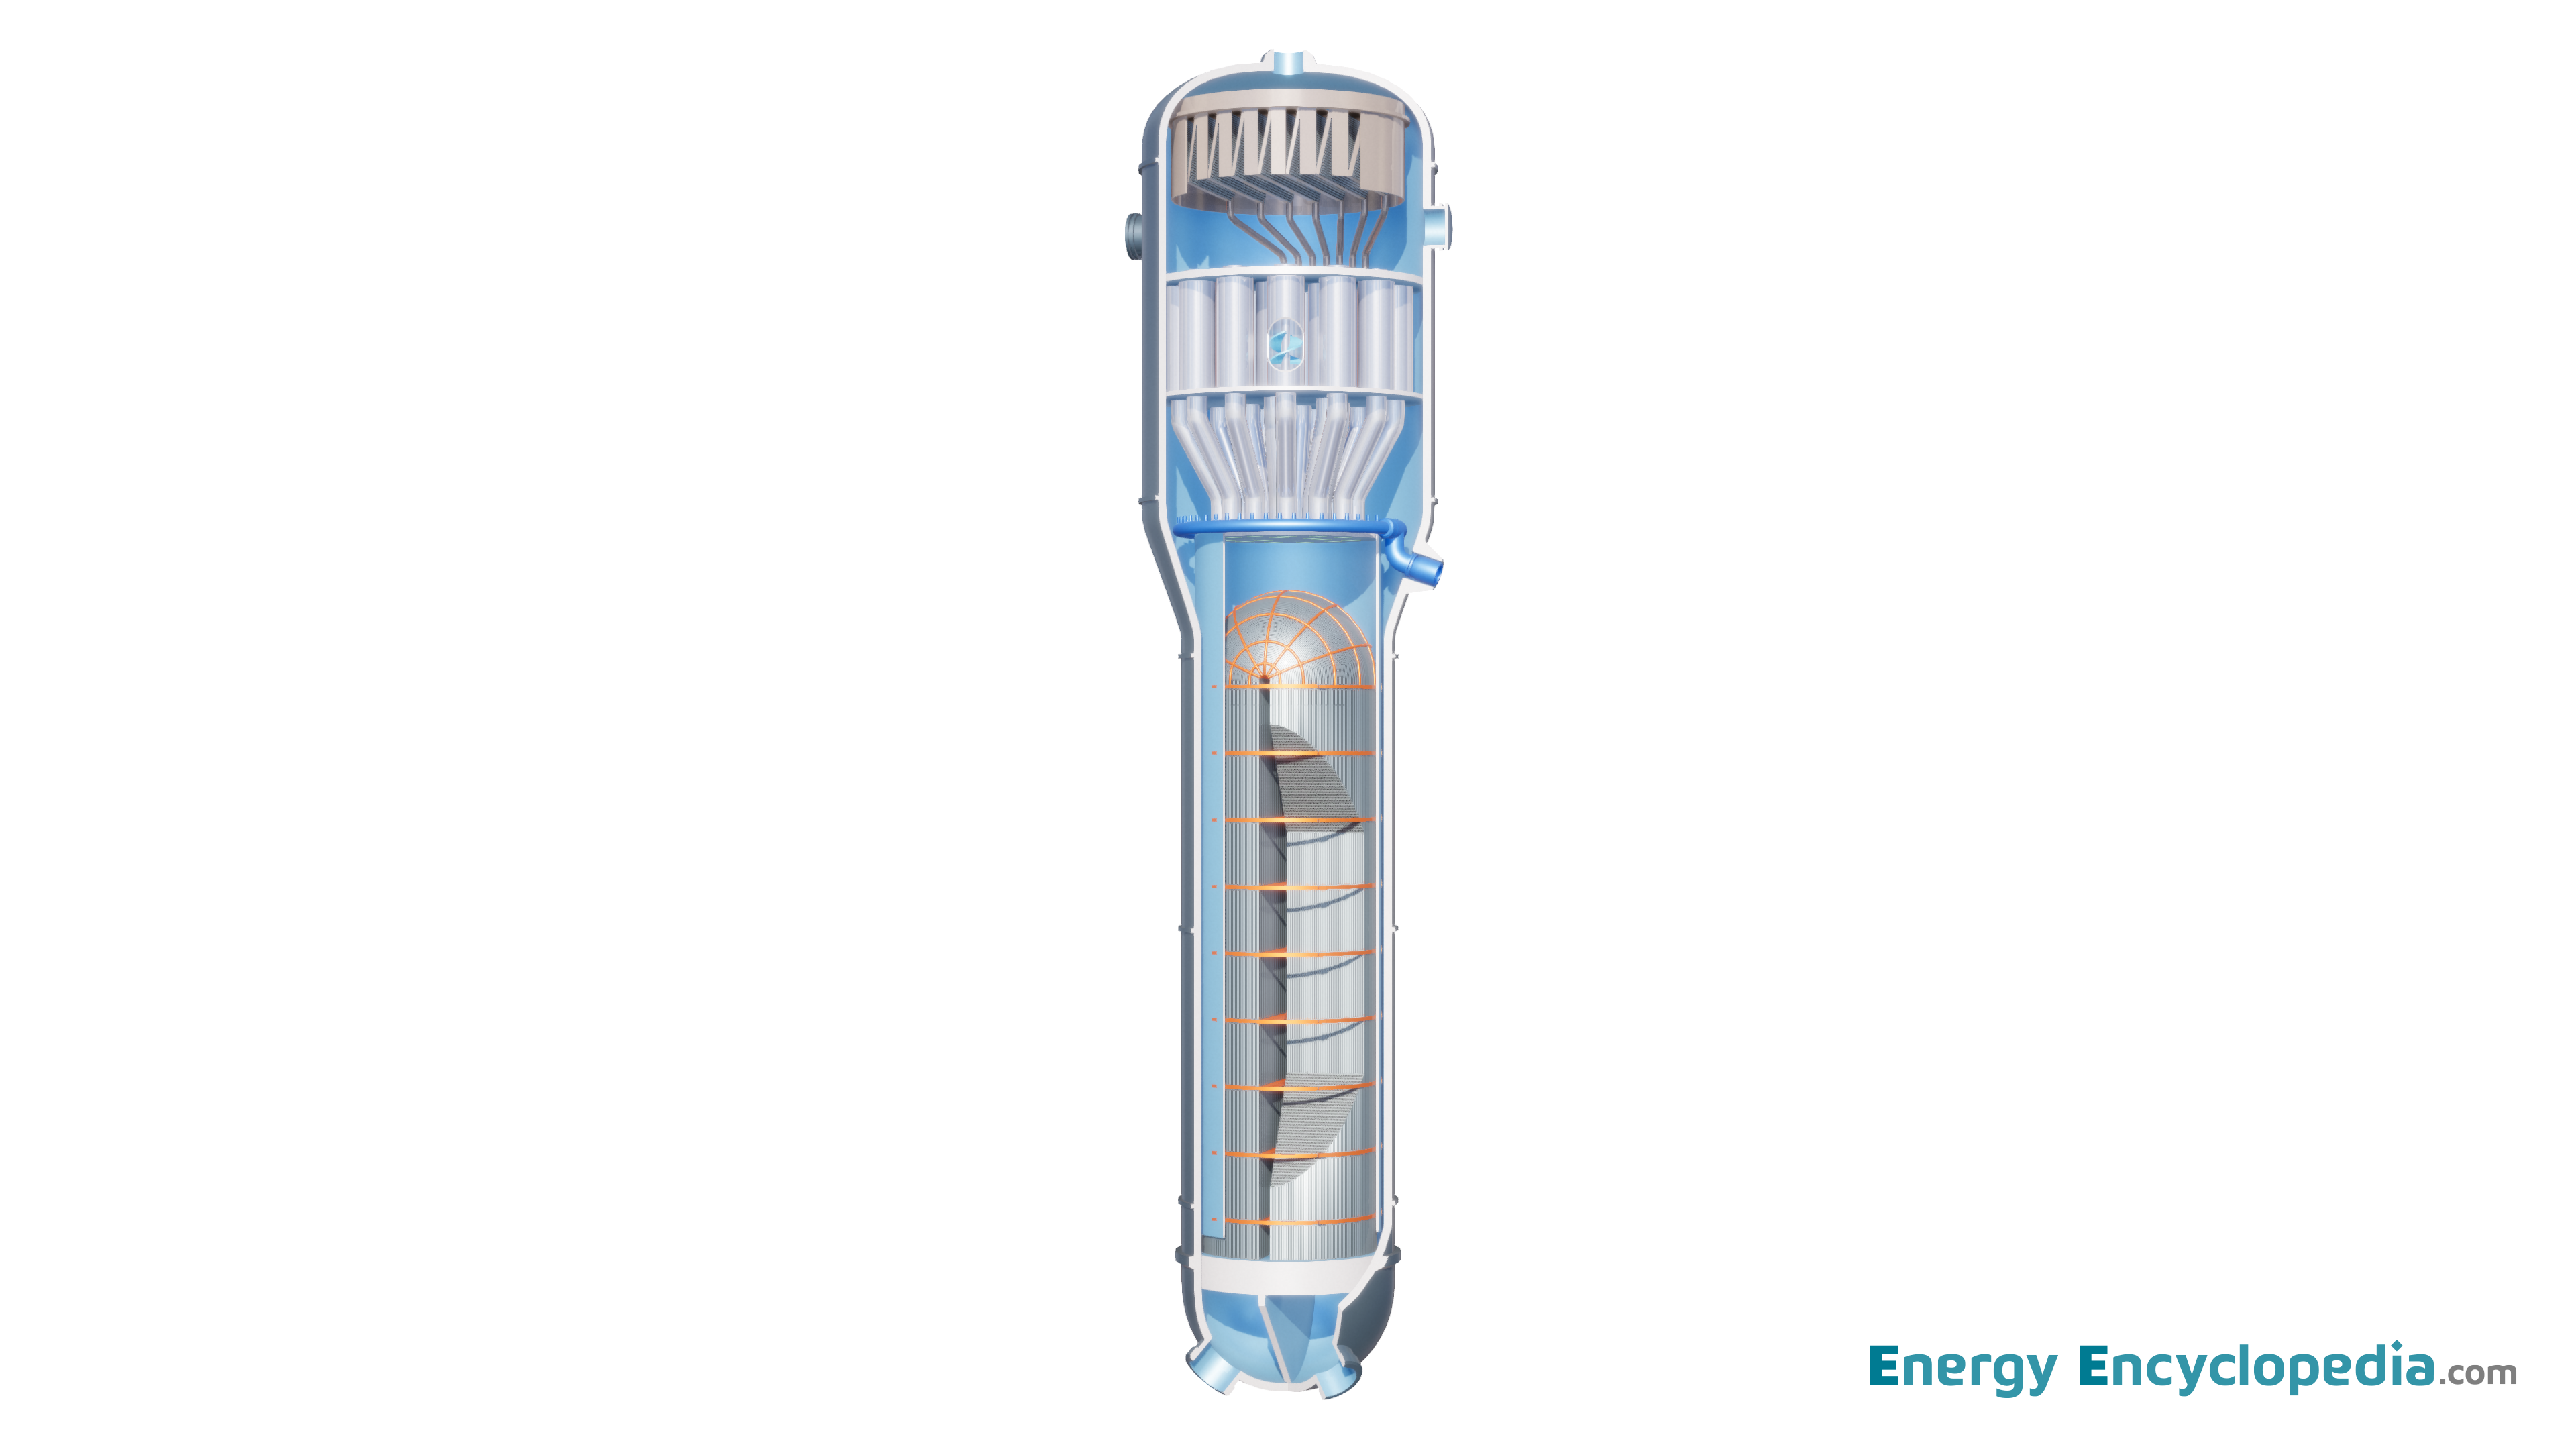
\includegraphics[width=\textwidth]{imgs/SG_PWR.png}
        \\[4pt]
        \footnotesize (a) \gls{pwr} steam generator
    \end{minipage}
    \hfill
    \begin{minipage}[b]{0.48\textwidth}
        \centering
        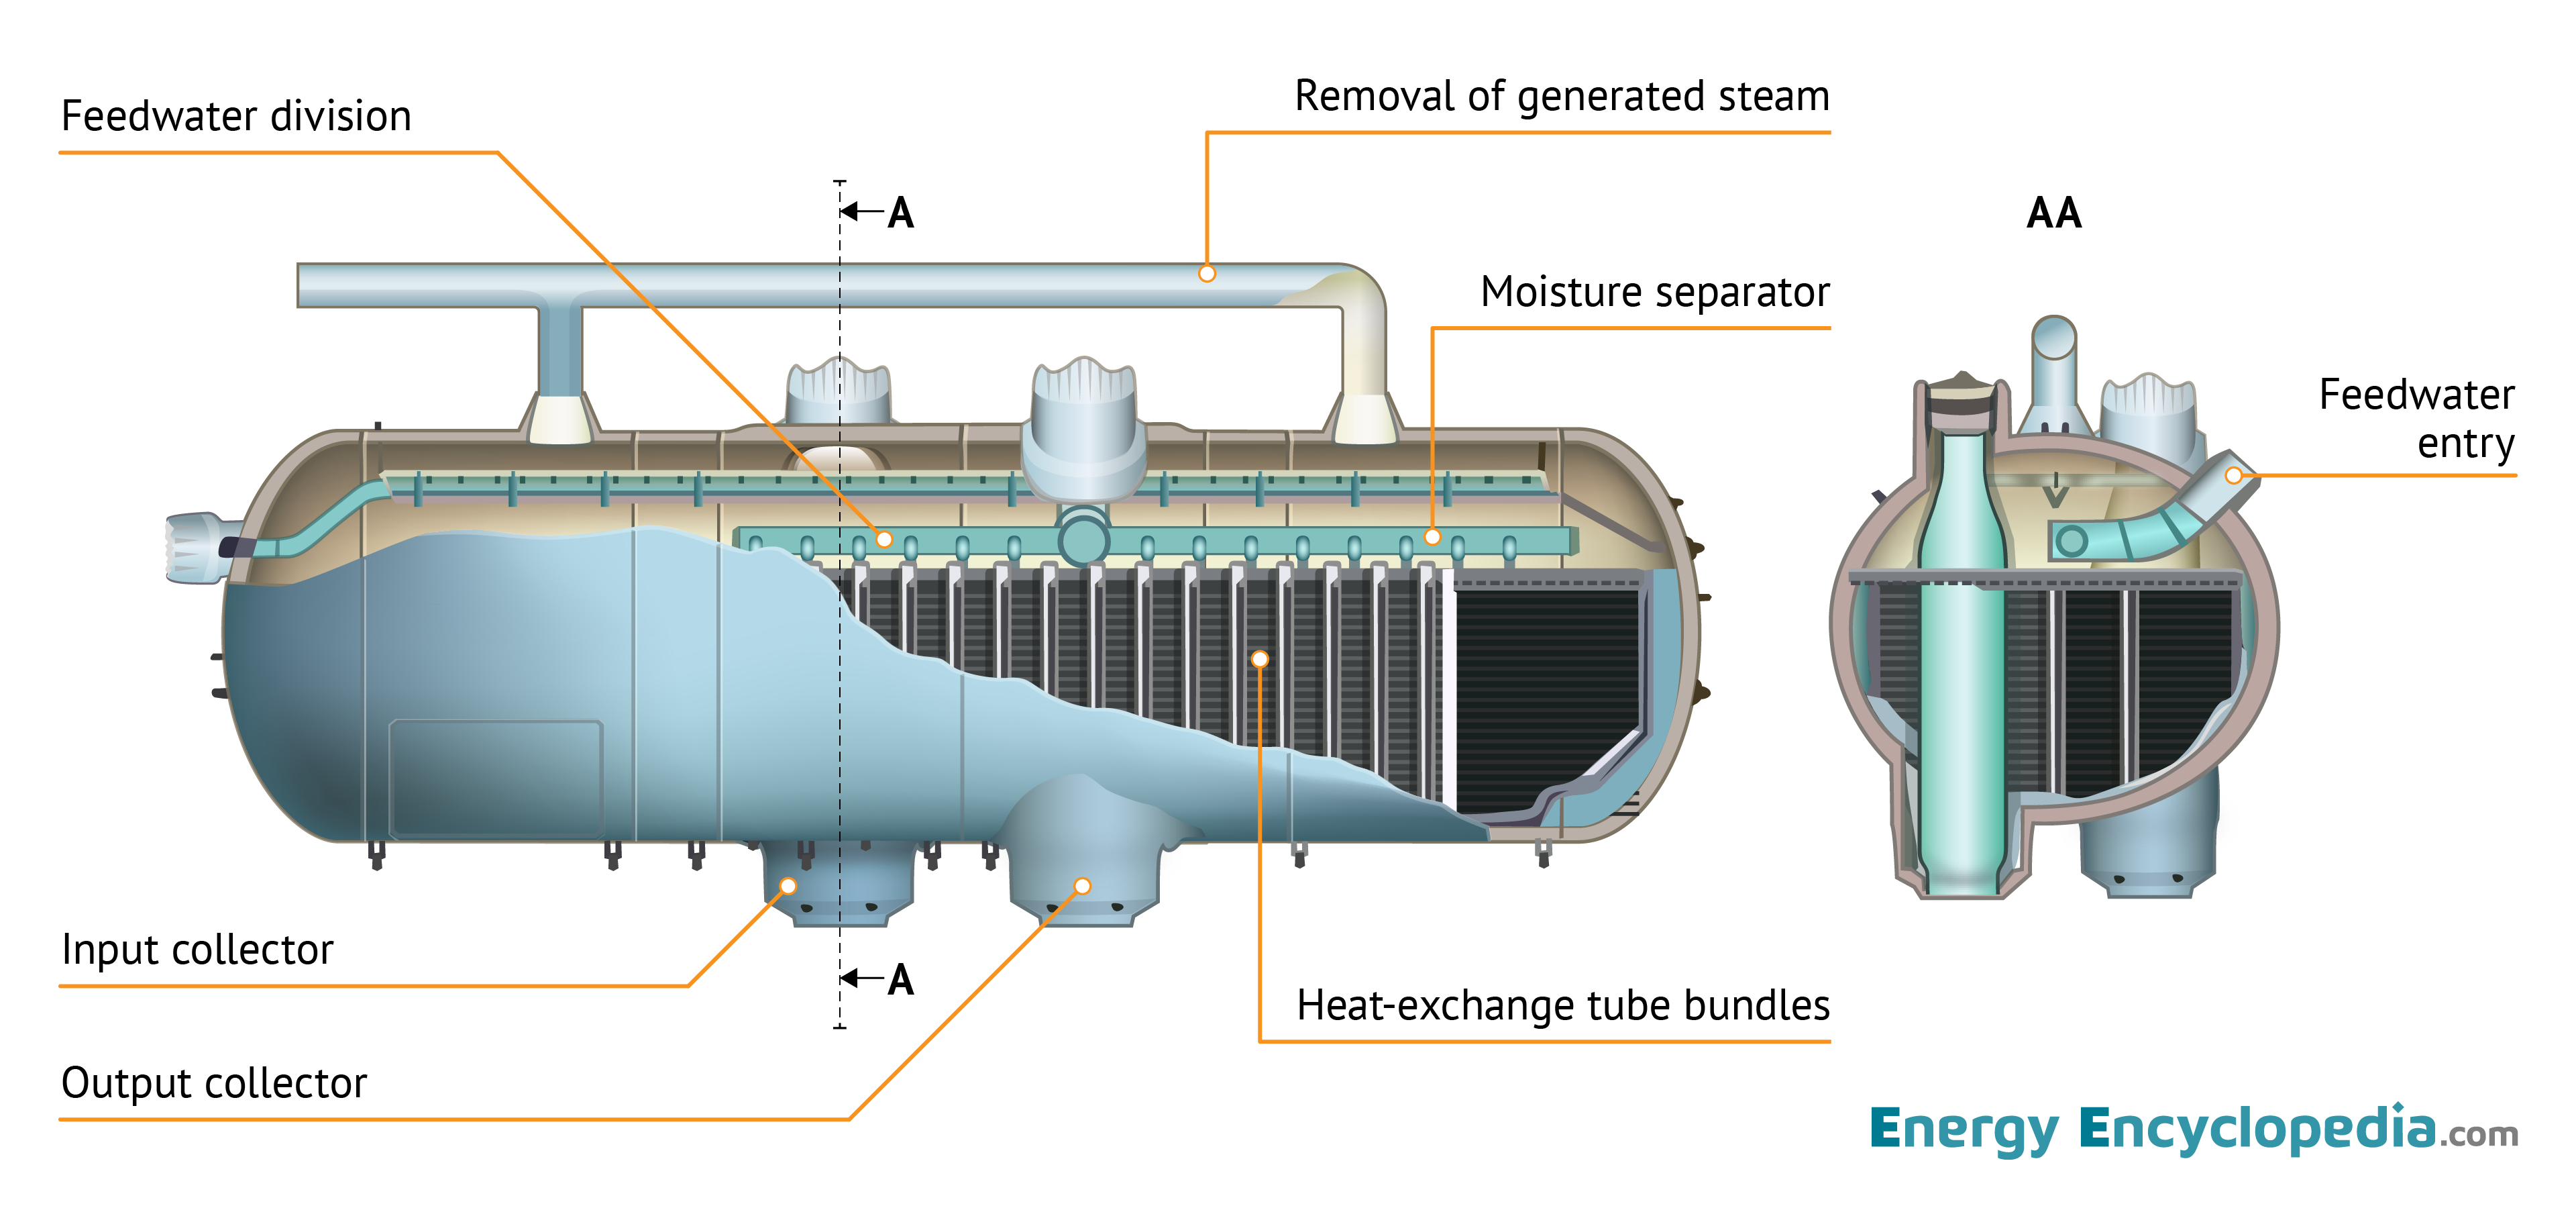
\includegraphics[width=\textwidth]{imgs/SG_VVER.png}
        \\[4pt]
        \footnotesize (b) \gls{vver} steam generator
    \end{minipage}
    \caption{Comparison of steam generator orientations in PWR (right, vertical) and VVER (left, horizontal) designs. Credit: energyencyclopedia.com}
    \label{fig:sg_orientations}
\end{figure}

Technological diversification occured also on other fronts as each nation developed its own reactor designs. The United Kingdom advanced gas-cooled Magnox reactors, the Soviet Union initiated development of the graphite-moderated, water-cooled RBMK design, while Canada's nuclear program focused on pressurized heavy water reactor (PHWR) technology, culminating in the first commercial CANDU reactor at Douglas Point in 1968 \cite{IAEA_PRIS_2025}.


\subsection{Generation II}
Between the 60s and 70s Generation II reactors were deployed, taking advantage of previous experience, reactors are now developed as commercial products rather then experiments or prototypes. In these decades numerous countries commissioned their first nuclear reactors: Belgium (1962), Italy (1963), Japan (1963), Sweden (1964), Switzerland (1969), Slovakia (1972), Argentina (1974), Bulgaria (1974) and Armenia (1976) \cite{IAEA_PRIS_2025}. Following the 1973 oil crisis, the deployment of nuclear power plants was accelerated in some countries as an energy security strategy. Most notably France implemented the Messmer Plan, named after the Prime Minister at the time, to greatly expand the nuclear plant fleet \cite{FundingUniverse_EDF_History_2025}. 

\begin{figure}[htbp]
    \centering
    
\includegraphics[width=0.7\textwidth]{imgs/placeholder.png}
    \caption{Map of first reactor deployments.}
    \label{fig:map_delopyments_npp}
\end{figure}

Nuclear expansion continued through the 1980s until 1986. As news from the Chernobyl disaster came to western countries, fear of the potential risks of nuclear power intensified. The public opposition grew significantly so that, even if safety and regulatory updates were implemented, several countries decided to slow down, reduce or halt their nuclear programs althogether, such was the case of Italy after the results of the 1987 referendum, which resulted in a complete phase-out of nuclear power \cite{MinisteroInterno_Referendum_1987, IAEA_PRIS_2025}. 

By the 1990s, multiple western countries had suspended nuclear deployment entirely, including Germany and Switzerland. France, previously the most active builder, connected 10 reactors between 1990-1999, while the United States and United Kingdom only deployed 4 and 1 reactors respectively during the same period. Italy completed its nuclear phase-out by 1990 with the permanent shutdown of all operating reactors \cite{IAEA_PRIS_2025}. 

Contrastingly, Eastern nations pursued an opposite trajectory. Following the post-Soviet economic transition, Russia resumed its nuclear program and has since continued expansion of its reactor fleet \cite{IAEA_PRIS_2025}. China initiated its nuclear program in the 1990s with Qinshan-1 (connected in 1991) and has since maintained aggressive expansion. Over the past three decades, China has brought 56 additional reactors online and currently has 29 under construction, positioning itself to surpass both France and the United States in total reactor capacity within the coming decade \cite{IAEA_PRIS_2025}.

\begin{figure}[htbp]
    \centering
    
\includegraphics[width=0.7\textwidth]{imgs/placeholder.png}
    \caption{Nuclear reactors deployment, per country throughout the years, with projections}
    \label{fig:npp_deployment_over_time}
\end{figure}

\subsection{Generation III}
As a result of the regulatory safety improvements, a stabilized choice of technology with LWRs settling as the to go choice all over the world and even larger capacities, Generation III reactor started to be developed in the 90s.

The improvement of these designs was fueled in the early 2000s by concerns over climate change, energy security, and rising fossil fuel prices, leading to Generation III+ reactors, such as the European Pressurized Reactor (EPR) or the US AP-1000 which improve safety and reliability in a consolidated plant layout. However after the 2011 Fukushima Daiichi accident, Western nations experienced a second setback: Germany accelerated its nuclear phase-out policy, while Italy reaffirmed its anti-nuclear position through another popular referendum \cite{MinisteroInterno_Referendum_2011}. In the following years projects faced substantial delays, cost overruns, and public opposition, with France's Flamanville-3 EPR serving as a particularly illustrative case experiencing budget increases to more then four times original estimates and construction timelines tripled from initial projections \cite{nea2020unlocking}.

\subsection{Generation IV}
From the late 2000s to nowadays, new nuclear commissioning projects such as Flamanville-3 can be classified as "Mega Projects", such term is used to refer to very large committments where economies of scale tend to fail due to the complexity of the task at hand, resulting in massive delays and cost overruns, well known examples of Mega Projects are Suez and Panama Canals, the Sydeny Opera House or the development of the Concorde Supersonic Aeroplane \cite{Flyvbjerg2014, BROOKES201557}. 

To counter this phenomena, the nuclear industry is developing Small Modular Reactors (SMRs) which are part of Generation IV reactors. SMRs are smaller, standardized reactors that can be built mostly off site to take advantage of economies of multiples. Some SMR designs are based on novelty technologies while others take advantage of well known water-based designs. 

Other generation IV reactors are being design to tackle on other aspects of nuclear power such as waste minimization or higher efficiencies. Manly by emplying different means of cooling to exploit neutrons at higher energies (fast neutrons), or by using thorium instead of uranium as fuel or even using direct gas based cycles to increase thermal efficiency.


\begin{figure}[htbp]
    \centering
    \begin{minipage}[b]{0.3\textwidth}
        \centering
        
\includegraphics[width=\textwidth]{imgs/placeholder.png}
        \\[4pt]
        \footnotesize (a) Gen IV example 1
    \end{minipage}
    \hfill
    \begin{minipage}[b]{0.3\textwidth}
        \centering
        
\includegraphics[width=\textwidth]{imgs/placeholder.png}
        \\[4pt]
        \footnotesize (b) Gen IV example 1
    \end{minipage}
        \hfill
    \begin{minipage}[b]{0.3\textwidth}
        \centering
        
\includegraphics[width=\textwidth]{imgs/placeholder.png}
        \\[4pt]
        \footnotesize (c) Gen IV example 1
    \end{minipage}
    \caption{Comparison of some gen IV designs}
    \label{fig:gen_IV_examples}
\end{figure}

\subsection{Current European Landscape}
In 2020, the COVID-19 pandemic exposed vulnerabilities in global economic systems and Russia's invasion of Ukraine in 2022 further revealed Europe's energy dependencies \cite{BRODNY2023121443, Sterling_European_Energy_Import_2025, EPRS_Energy_2023}. At the same time, decarbonization goals to combat climate change have prompted Western nations to reconsider nuclear energy as a valid power source able to provide low-carbon, reliable power while enhancing energy independence and system resilience \cite{EU2050ClimateStrategy}.

This strategic reassessment of nuclear is evident in recent policy initiatives. The European Union's classification of nuclear power as a sustainable investment under its taxonomy for climate mitigation \cite{EUTaxonomy}, alongside programs like the European Industrial Alliance on \glspl{smr} are a clear indicator of the renewed interest in nuclear technologies.

\textcolor{red}{I might add more...}

\section{Decision Support}
The historical overview demonstrates that nuclear energy decisions extend far beyond technical and economic considerations, inevitably encompassing social and political dimensions. This inherent complexity requires \glspl{dm} to evaluate numerous trade-offs across competing objectives in pursuit of balanced, optimal solutions. The systematic process of navigating trade-offs to arrive at informed choices constitutes the fundamental challenge of decision-making.

The decision making process begins by identifying the decision problem and the possible solutions to such problem. From this point, there are several ways to take the decision. The most common approach to decision making, which is encountered by anyone in our day to day life, is to look at the possible solutions or "alternatives", compare positive and negative outcomes based on own preferences and find the best, or less worst, between them.

For more complex situations such as those regarding energy systems, analytical frameworks, usually referred to as \gls{dss}, have been developed to support \glspl{dm}. In the realm of business and management \glspl{dss} are widely employed as softwares that collect and organize data, communications or knowledge to provide support by data analyses or visualization or by applying models. \cite{Power2023}.

The present study is focused on nuclear energy related decisions. The literature review will reveal that \gls{mcda} methods predominate in energy decision support research. This observation aligns with findings from Seran et al. (2025), whose comprehensive analysis of renewable energy studies demonstrated that the vast majority employed \gls{mcda} methodologies \cite{SERAN2025100044}.

\gls{mcda} systematically evaluates alternative solutions by decomposing decision problems into distinct criteria representing either the consequences of each alternative or their distinguishing characteristics \cite{ROY1990324}. This criterion-based approach offers two primary advantages: first, it enables the structured analysis of complex problems involving many criteria; second, it reveals preference patterns from different perspectives, which becomes particularly valuable when multiple stakeholders are involved. The method's transparency allows decision-makers to identify the most critical aspects of each alternative in relation to specific stakeholder preferences.

While there exists many \gls{mcda} methodologies (see Greco et Al. 2016 \cite{Köksalan2016} and Cinelli et al. 2020 \cite{CINELLI2020102261}) their common ground is to model the decision problem considering all availble information on it, considering trade-offs and then allowing to choose between alternatives \cite{HAAG2022105361}. \gls{mcda} can be used for solving different decision problems:
\begin{itemize}
\item Choice: Selecting the most preferred alternative(s) from a large pool of options.
\item Sorting: Classifying alternatives into predefined categories.
\item Ranking: Ordering all alternatives from most to least preferred.
\item Scoring: Ranking alternatives while also quantifying the differences between them.
\end{itemize}

A fundamental distinction exists between American and European \gls{mcda} methodologies. American-developed approaches, including the \gls{ahp} and \gls{mavt}, were born on the basis of the compensatory principle, emphasizing trade-off dynamics where a loss in one criterion can be offset by a gain in another.

In contrast, European researchers developed non-compensatory methods based on the outranking principle, such as ELECTRE and PROMETHEE. These methods establish preferences through binary outranking relationships between alternatives (e.g., "alternative A1 is preferred to A2 on regard to criterion C1") and may incorporate veto conditions between criteria. Unlike compensatory approaches, outranking methods were focused on meeting requirements rather than optimizing trade-offs \cite{HUANG2026103438, Köksalan2016}.

\section{Relevant Studies}
A review of relevant literature reveals numerous applications of MCDA methods across diverse fields. Focusing specifically on studies combining MCDA with nuclear power decision-making, several distinct approaches emerge:

Site selection studies represent the most common application, typically employing GIS-based software to evaluate potential locations for new nuclear installations within limited geographical regions. These analyses frequently incorporate quantitative non-technical factors such as population proximity \cite{DAMOOM2019110} \cite{BASEGMEZ2025105897}. Abdullah et al. (2025) extend this approach by including social dimensions like public acceptance and tourism impacts, which present challenges for quantification \cite{ABDULLAH2025105626}. Notably, Devanand et al. (2019) develop an algebraic optimization model to identify optimal SMR locations in Singapore, though like most site-focused studies, they favor a design without sistematic comparison \cite{DEVANAND2019339}.

A second category compares different nuclear technologies. Kiser and Otero (2023) evaluates PWRs, SMRs, and Molten Salt Reactors \cite{KISER2023104647}, while Locatelli and Mancini (2011) compares large and small reactor designs \cite{Locatelli01092012}. Birikorang's study stands out for its regional focus on South Africa and comparison of three specific reactor models (NuScale SMR, EM2-HTGR, FTR-MSR), though its technological comparisons mix designs at different maturity levels \cite{BIRIKORANG2026111837}. Notably, all three studies utilize the Analytic Hierarchy Process (AHP) or its Fuzzy variant. The last one (Birikorang) draws on the IAEA's INPRO methodology for advanced nuclear technology comparison \cite{IAEA_INPRO_2019}.

Broader energy comparison studies by Hernández-Torres (2025), Pasaoglu (2018), and Atilgan (2016) evaluate multiple generation options (typically eight alternatives) employing AHP-TOPSIS, AHP, and MAVT methodologies respectively. These studies use generic, averaged parameters for each technology class \cite{HERNANDEZTORRES2025122481,PASAOGLU2018654,ATILGAN2016168}. In contrast, Castelazo (2014) adopts a more precise approach using Multi-Attribute Value Theory (MAVT) to compare thirteen energy technologies, employing specific reference plants (e.g. EPR reactor for nuclear power) rather than generalized technology averages \cite{SANTOYOCASTELAZO2014119}.

Three studies show particular relevance to the current research. Zolkaffly et al. (2014) evaluates nuclear plant models in Malaysia but suffers from outdated data and neglects non-technical aspects \cite{10.1063/1.4866099}. Topaloğlu (2025) applies the Analytic Network Process (ANP) to compare reactor types (PWR, BWR, PHWR) and locations, though social considerations remain limited to site-specific factors \cite{TOPALOGLU2025103228}. Goushis (2025) employs TOPSIS to assess SMR deployment in the EU for coal replacement, but focuses on a single reactor model rather than comparative technology evaluation \cite{GOUSHIS2025126565}.

The literature review reveals four gaps in nuclear energy decision-making research. First, most studies focus solely on site selection rather than comparing different nuclear technologies. Second, comparisons between nuclear designs lack consideration of a specific decision-making context. Third, studies that do consider specific decision-making context, examine various energy generation options as broad technology categories (e.g., nuclear, solar, wind) rather than conducting detailed analyses of specific power plant designs. Fourth, social dimensions are frequently overlooked or applied only to site selection criteria.

\section{Observation on the validity of public surveys}
During this study's execution, multiple public surveys were reviewed based on the initial assumption that such instruments could provide quantitative measurements of qualitative factors such as public support for nuclear installations. However, the analysis exposed frequent methodological limitations introducing bias into the results. In Italy, a 2024 IPSOS survey commissioned by Legambiente (an environmental NGO with a known anti-nuclear position) reported 81\% opposition to nuclear power \cite{IPSOS_Nuclear_Survey_2024}. However, analysis of the survey report reveals problematic question design. The primary question was phrased as: \textit{"The debate on nuclear energy has returned to the forefront. What is your opinion on the matter?"} with response options structured as:
\begin{itemize}
    \item A1: "The current situation is complex; a return to nuclear should be evaluated"
    \item A2: "Nuclear has more risks than benefits and is not the right path"
    \item A3: "Nuclear energy entails excessive hidden costs and is not advantageous"
    \item A4: "Only safer technologies than current ones should be considered"
\end{itemize}

This framing demonstrates clear bias: two options (A2 and A3) explicitly oppose nuclear, A1 offers only conditional support, and A4 introduces safety concerns before suggesting potential support. Notably, the 81\% opposition figure includes A4 responses, which represent conditional rather than absolute opposition. When considering only explicit opposition (A2+A3), the figure decreases to 43\%.\\

A 2024 SWG study presents a more methodologically sound approach, though its conference presentation emphasized positive findings. The actual data reveals a more nuanced picture: over 80\% of respondents consider themselves insufficiently informed about nuclear topics, and further investigation found that approximately 90\% were unaware of SMRs or Generation IV reactors \cite{SWG_Nuclear_Survey_2024}. These findings suggest that public opinion on nuclear energy may be more influenced by lack of information than by firmly held positions.